% Figure: three pressures on a proven design (part 1).
% Build: pdflatex three_pressures.tex  (run inside figures/)
\documentclass[tikz,border=6pt]{standalone}
\usetikzlibrary{positioning,arrows.meta}
\begin{document}
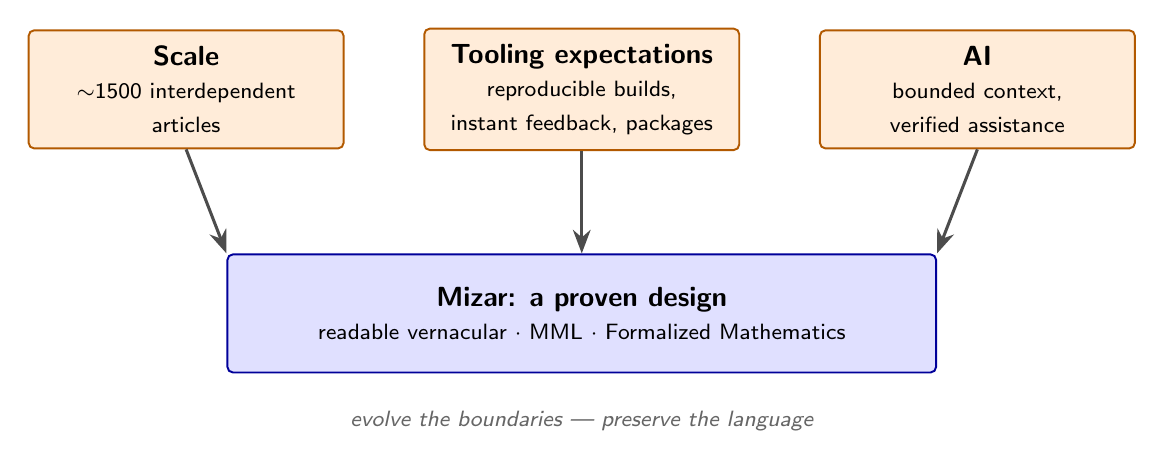
\begin{tikzpicture}[
  font=\sffamily,
  pressure/.style={draw, rounded corners=2pt, align=center, minimum width=40mm,
                   minimum height=15mm, line width=0.7pt, inner sep=2mm},
  flow/.style={-{Stealth[length=3mm]}, line width=1.1pt, black!70},
  note/.style={font=\sffamily\footnotesize\itshape, text=black!60, align=center},
]
  \node[pressure, fill=orange!15, draw=orange!70!black] (scale)
    {\textbf{Scale}\\ \footnotesize $\sim$1500 interdependent\\ \footnotesize articles};
  \node[pressure, fill=orange!15, draw=orange!70!black, right=10mm of scale] (tool)
    {\textbf{Tooling expectations}\\ \footnotesize reproducible builds,\\ \footnotesize instant feedback, packages};
  \node[pressure, fill=orange!15, draw=orange!70!black, right=10mm of tool] (ai)
    {\textbf{AI}\\ \footnotesize bounded context,\\ \footnotesize verified assistance};

  \node[pressure, fill=blue!12, draw=blue!60!black, minimum width=90mm,
        below=13mm of tool] (mizar)
    {\textbf{Mizar: a proven design}\\
     \footnotesize readable vernacular \(\cdot\) MML \(\cdot\) Formalized Mathematics};

  \draw[flow] (scale.south) -- (mizar.north west |- mizar.north) ;
  \draw[flow] (tool.south) -- (mizar.north);
  \draw[flow] (ai.south) -- (mizar.north east |- mizar.north);

  \node[note, below=3.5mm of mizar]
    {evolve the boundaries --- preserve the language};
\end{tikzpicture}
\end{document}
